\begin{figure}
    \begin{center}
    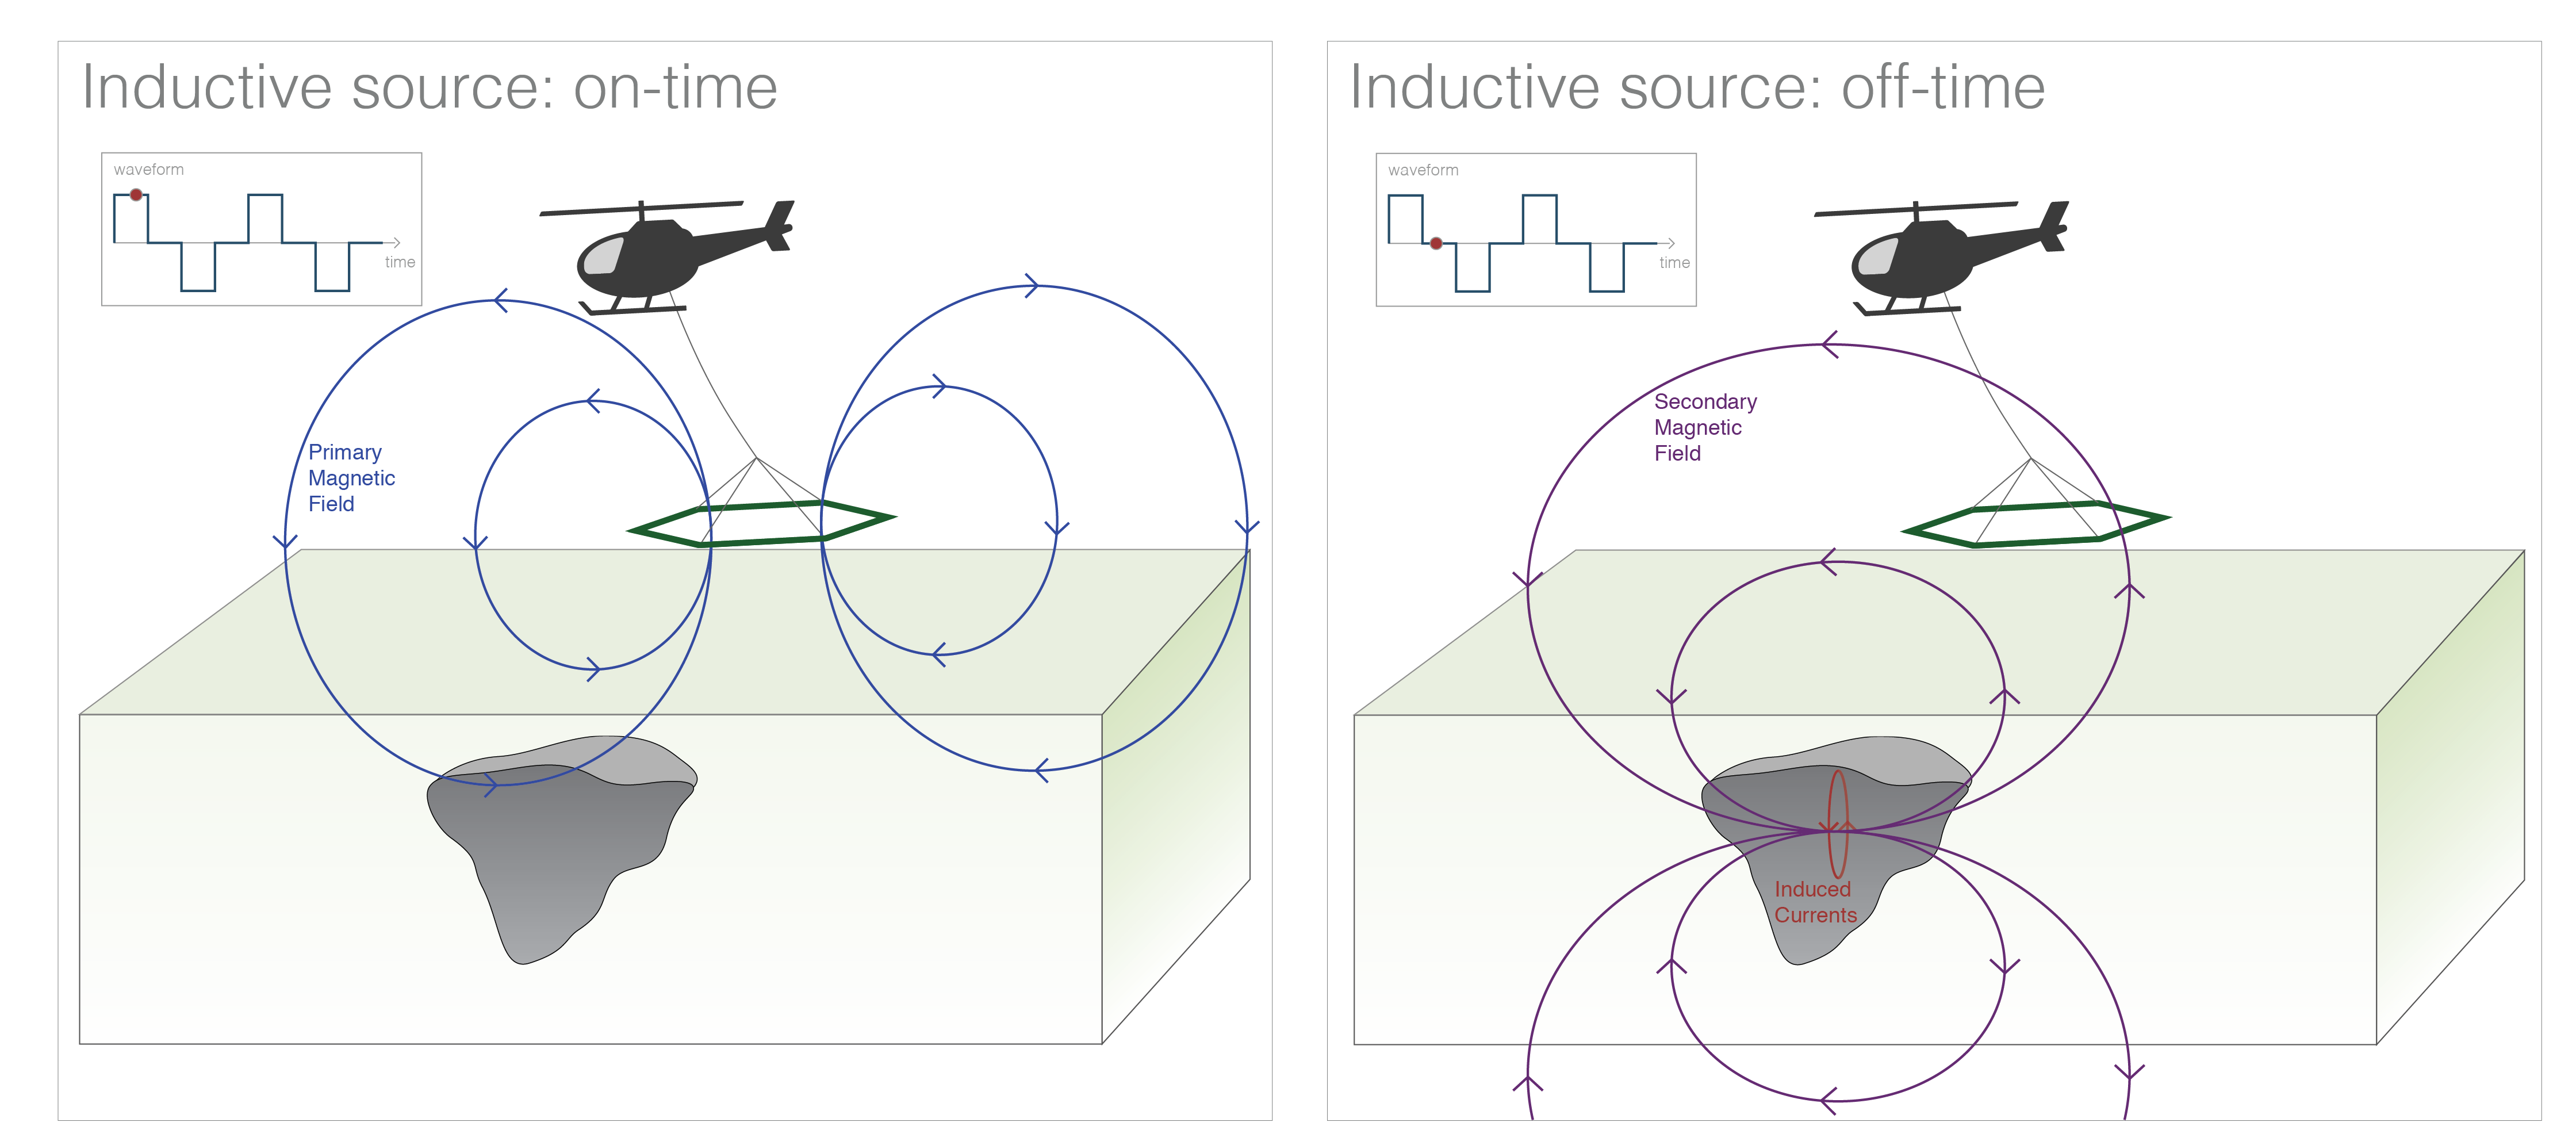
\includegraphics[width=\textwidth]{figures/intro/inductive-sources.png}
    \end{center}
\caption{
    Time-domain inductive source experiment. (Left) a steady-state current is passed through the transmitter loop, generating a primary magnetic field. (Right) This current is shut-off, causing a change in magnetic flux. The changing magnetic flux induces secondary currents in conductors, which in turn create secondary magnetic fields that can be measured at receivers above, on, or within the earth.
}
\label{fig:inductive-sources}
\end{figure}
